\documentclass[10pt,a4paper]{article}

%-------------------------------%
% Commands and packages
\usepackage{amsmath,amssymb,bm,physics,graphicx,hyperref}
\usepackage{subcaption}
\usepackage[backend=biber, style=ieee]{biblatex}

\hypersetup{
    colorlinks = true,  %Colours links instead of ugly boxes
    urlcolor   = blue,  %Colour for external hyperlinks
    linkcolor  = black, %Colour of internal links
    citecolor  = black  %Colour of citations
}

%-------------------------------%
% Main document
\begin{document}
    \numberwithin{equation}{section}
    \numberwithin{table}{section}
    \section{Dynamic System Analysis}
    The aircraft system dynamics is described by the following set of differential equations (which are linear and already in state space representation). State variables are $\alpha, r, \theta$ and input variable is $\delta$.
    \begin{subequations}
        \begin{align}
            \dot{\alpha} =& -0.31\alpha + 57.4r +0.232\delta, \\
            \dot{r} =& -0.016\alpha-0.425r+0.0203\delta, \\
            \dot{\theta} =& 56.7r.
        \end{align}
    \end{subequations}
    The 3 transfer functions describing aircraft system dynamics:
    \begin{subequations}
        \begin{align}
            G_{\alpha}(s) =& \frac{A(s)}{\Delta(s)}, \\
            G_{r}(s) =& \frac{R(s)}{\Delta(s)}, \\
            G_{\theta}(s) =& \frac{\Theta(s)}{\Delta(s)}.
        \end{align}
    \end{subequations}
    For open-loop dynamics, we must take into account the impact of the actuator and sensor. From the question sheet, we know the actuator has transfer function
    \begin{subequations}
        \begin{align}
            G_{a}(s)=\frac{1}{0.0145s+1}, \label{eq:tf_actuator}
            \intertext{and the sensor has transfer function}
            G_{m}(s)=\frac{e^{-0.0063s}}{0.0021s+1}. \label{eq:tf_sensor}
        \end{align}
    \end{subequations}
    We assume that the system has zero initial conditions when determining these transfer functions. Given the transfer functions of the actuator, Equation (\ref{eq:tf_actuator}) and sensor, Equation (\ref{eq:tf_sensor}) in this system, we can find that the poles of both have negative real parts $s = -\frac{1}{0.0145}$, $s=-\frac{1}{0.0021}$ respectively; and are therefore stable. Since the open-loop system is the cascade of the actuator, aircraft dynamics, and sensor as shown in the block diagram in Figure \ref{fig:blockDiagram}. Provided the transfer function relating to the aircraft dynamics ($G_{\alpha}, G_{r}, G_{\theta}$) has only poles with negative real parts, the open-loop system will be stable.
    \begin{figure}[h]
        \centering
        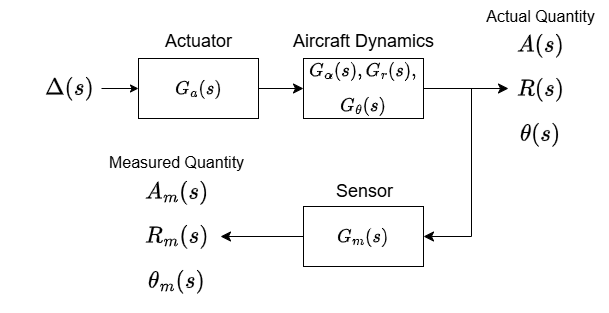
\includegraphics[width = 0.75\textwidth]{figs/ELE2038_H5.drawio.png}
        \caption{A block diagram of the control system.}
        \label{fig:blockDiagram}
    \end{figure}
    
    \subsection{Analysis of $G_{\alpha}, G_{r}, G_{\theta}$.}
    From the system of differential equations the transfer functions of $G_{\alpha}$, $G_{r}$ and $G_{\theta}$ can be derived.
    \begin{subequations}
        \begin{align}
            G_\alpha =& \frac{0.232s + 1.26382}{(s + 0.31)(s + 0.425) + 0.9184} \\
            G_r =& \frac{0.0203s + 0.002581}{(s + 0.31)(s + 0.425) + 0.9184} \\
            G_\theta =& \frac{1.15101s + 0.1463427}{s((s + 0.31)(s + 0.425) + 0.9184)}
        \end{align}
    \end{subequations}
    The poles of $G_\alpha$ occur when $s^{2}+0.735s+1.05015=0$ which can be solved using the quadratic formula to give $s=-0.3675 \pm j0.9566$. The poles of $G_r$ also occur when $s^{2}+0.735s+1.05015=0$ and therefore result in the same value. Since $G_{\theta}(s)=\frac{56.7}{s}G_{r}(s)$; $G_{\theta}(s)$ shares all of the poles of $G_{r}(s)$, which are all stable, but also possesses an additional pole at $s=0$. This means the poles of $G_{\theta}(s)$ are $s=-0.3675 \pm j0.9566, s=0$. Since we have a pole with a non-negative real part, $G_{\theta}$ is not BIBO stable, meaning the open-loop system relating deflection angle of elevators to pitch angle is also not BIBO stable. This means a controller will be required to obtain BIBO stability of the system.
    \begin{figure}
    \centering
        \begin{subfigure}[h]{0.5\textwidth}
            \centering
            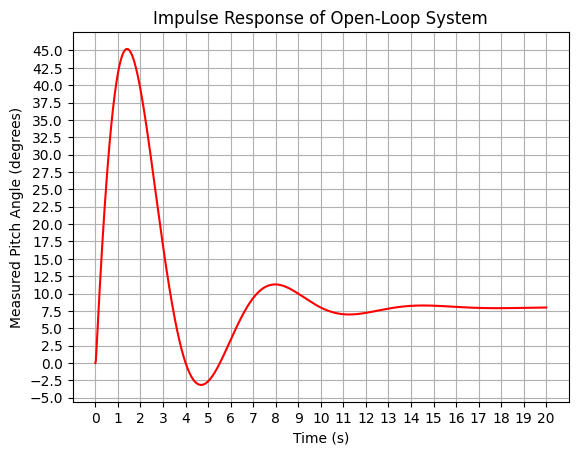
\includegraphics[width = \textwidth]{figs/GthetaImpRes.png}
            \caption{The impulse response of $G_\theta$.}
            \label{fig:gThetaImpRes}
        \end{subfigure}%
        \begin{subfigure}[h]{0.5\textwidth}
            \centering
            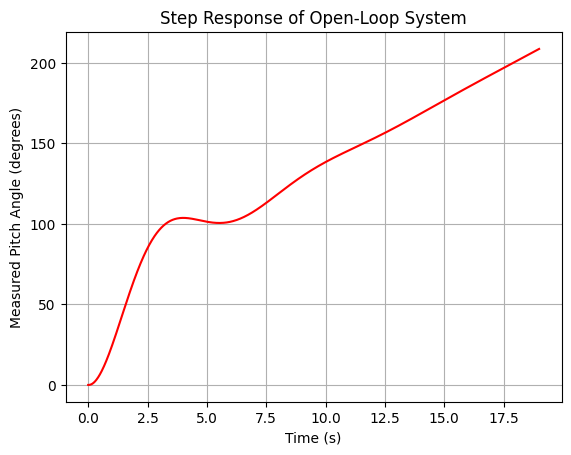
\includegraphics[width = \textwidth]{figs/GthetaStepRes.png}
            \caption{The step response of $G_\theta$.}
            \label{fig:gThetaStepRes}
        \end{subfigure}
    \caption{Output plots of $G_\theta$.}
    \end{figure}
    Figure \ref{fig:gThetaImpRes} shows that when the deflection angle of the elevators $\delta$ is a unit impulse, the pitch angle $\theta$ of the aircraft reaches a maximum of roughly 45 degrees after 1.5 seconds, before stabilising at (roughly) 7.5 degrees after around 16 seconds. Note that despite the input being a unit impulse, the pitch angle does not return to zero for the open-loop system.    Figure \ref{fig:gThetaStepRes} shows that as time increases, pitch angle $\theta$ is increasing unbounded. This follows from the prior discovery that $G_{\theta(\text{open-loop})}$ is not BIBO stable. The frequency response of $G_\theta$ is plotted along with the impulse, step and frequency responses of $G_\alpha$ and $G_r$ in the attached Python notebook.    
\end{document}